El \textit{análisis de componentes principales} (PCA\footnote{\textit{Principal component analysis} en inglés.}) es un procedimiento estadístico ampliamente empleado para la reducción de dimensiones de un conjunto de datos.

La \textit{covarianza} mide la dependencia lineal entre dos variables aleatorias $x,y\in \mathbb{R}^n$.
Valores muy grandes o muy pequeños indican una fuerte dependencia entre las variables, respectivamente directa (a grandes valores de una corresponden grandes valores de la otra) o inversa (a grandes valores de una corresponden pequeños valores de la otra).
Puede calcularse como:

\begin{equation}
    \label{eq:covariance}
    \sigma_{x,y} = \frac{1}{n}\sum_{i=1}^{n}{(x_i - \bar{x})(y_i - \bar{y})}
\end{equation}

En un conjunto de datos, cada componente de sus elementos puede ser considerada desde el punto de vista estadístico como una variable aleatoria, y por tanto usada para el análisis de las covarianzas entre ella y el resto de componentes.
Para ello se construye la llamada \textit{matriz de covarianza}, que tiene la siguiente forma:

\begin{equation}
    \label{eq:covariance-matrix}
    \Sigma_X = \begin{bmatrix}
                   \sigma_{1,1} & \sigma_{1,2} & \ldots & \sigma_{1,m} \\
                   \sigma_{2,1} & \sigma_{2,2} & \ldots & \sigma_{2,m} \\
                   \vdots & \vdots & \ldots & \vdots \\
                   \sigma_{m,1} & \sigma_{m,2} & \ldots & \sigma_{m,m}
    \end{bmatrix}
\end{equation}

\noindent
donde $\sigma_{i,j}$ es el valor de la covarianza entre las componentes $i$ y $j$ del conjunto de datos $X$.

Los valores en las diagonales de la matriz corresponden a la varianza de cada una de las dimensiones.

El conjunto de datos de $n$ elementos puede representarse situando estos en las filas de una matriz $X$, que por tanto tiene $n$ filas y $m$ columnas.
Si se preprocesa dicha matriz restando a cada valor la media de su columna, cada atributo tendrá media 0, y se cumplirá $\Sigma_X = X^T X$~\cite{Tan05}.

El objetivo del PCA es transformar el conjunto de datos a un espacio donde las componentes sean linealmente independientes unas de otras.
Para ello, se busca que se cumplan las siguientes propiedades:

\begin{enumerate}
    \item Cada par de atributos diferentes tiene covarianza 0.
    En otras palabras, la matriz de covarianza de los datos transformados debe ser una matriz diagonal.
    \item Los atributos se encuentran ordenados respecto a la cantidad de varianza de los datos que cada uno contiene.
\end{enumerate}

Se puede obtener una transformación de los datos que cumpla dichas propiedades a partir de los valores y vectores propios de la matriz de covarianza.
Sean $\lambda_1,\dots,\lambda_m$ los valores propios de $\Sigma_X$.
Puesto que la matriz de covarianza es semidefinida positiva, todos los valores propios son no negativos, y pueden ser ordenados de modo que se cumpla $\lambda_1 \geq \lambda_2 \geq \dots \geq \lambda_{m-1} \geq \lambda_m$.
Sea asimismo $U = [u_1,\dots,u_m]$ matriz donde cada columna $u_j$ es un vector propio de $\Sigma_X$, dispuestos de forma que el $j$-ésimo vector corresponde al $j$-ésimo valor propio más grande.
Luego, asumiendo que la media de cada atributo de la matriz $X$ es 0, se cumple que~\cite{Smith02,Tan05}:

\begin{itemize}
    \item La matriz $\hat{X} = XU$ es la matriz correspondiente al conjunto de datos transformado, que cumple las condiciones mencionadas anteriormente.
    \item Cada nuevo atributo es una combinación lineal de los atributos originales. Específicamente, los pesos de la combinación lineal correspondiente al $j$-ésimo atributo son las componentes del $j$-ésimo vector propio.
    \item La varianza del $j$-ésimo atributo es $\lambda_j$.
    \item La suma de las varianzas de los atributos originales es igual a la suma de las varianzas de los nuevos atributos.
\end{itemize}

Los nuevos atributos son conocidos como \textbf{componentes principales}, y usualmente diferentes criterios pueden utilizarse para reducir la cantidad de dimensiones a partir de estas.
Puesto que la cantidad de varianza decrece con cada componente principal, usualmente basta con seleccionar solamente las primeras hasta cierta posición.
Una variante muy popular para decidir la cantidad de componentes principales a mantener (y por ende la cantidad de dimensiones del conjunto de datos transformado), es seleccionarlas hasta el punto en que la suma de sus varianzas sobrepasa una fracción predefinida de la varianza total (por ejemplo, el 95\%).

\begin{figure}[!h]
    \centering
    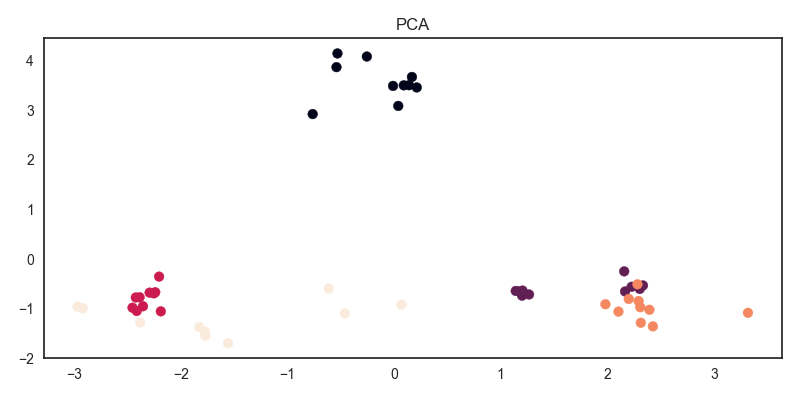
\includegraphics[width=0.85\textwidth]{pca.png}
    \caption{Resultado de aplicar PCA para reducir a dos las dimensiones de los MFCC de un conjunto de sonidos de 5 especies animales.}
    \label{img:pca}
\end{figure}
